\newpage
\section{Functionalități}

În acest capitol sunt prezentate funcționalitățile implementate in aplicația dezvoltată. Aplicația afișează o diagrama 
care are la baza un model 3D format din mai multe elemente.\newline

Functionalități de bază:
\begin{itemize}
    \item încărcarea oricarui fisier .mdef și crearea diagramei
    \item modificarea diagramei create
    \begin{itemize}
        \item mutarea elementelor
        \item scalarea intregii diagrame
        \item schimbarea culorii anumitor elemente
    \end{itemize} 
    \item salvarea modificarilor într-un fisier separat
    \item încărcarea automata a fișierului salvat, dacă există
    \item afisarea modelului din mai multe perspective ortografice
    \item afisarea modelului sub forma de graf
    \item căutarea unui element dupa un cuvant cheie și evidențierea lui
    \item compararea dintre diferite versiuni de modele
    \item afișarea unui panou de tip legendă care prezintă diferitele tipuri de elemente
    \item afișarea unui panou de informatii în care sunt afisate informații aditionale legate de elemente selectate
\end{itemize}

Se pot încărca oricâte fișiere .mdef în aplicație, fiecare fișier fiind reprezentat într-un tab diferit. 
Acest lucru se face din file->open, unde se v-a deschide o noua fereastra de unde utilizatorul își poate alege fișierul. 
Odată ales un fișier el este deschis într-un tab nou care conține o scena cu mai multe elemente de tip Motion body, 
Joint sau Connector.\newline

\begin{figure}[h]
    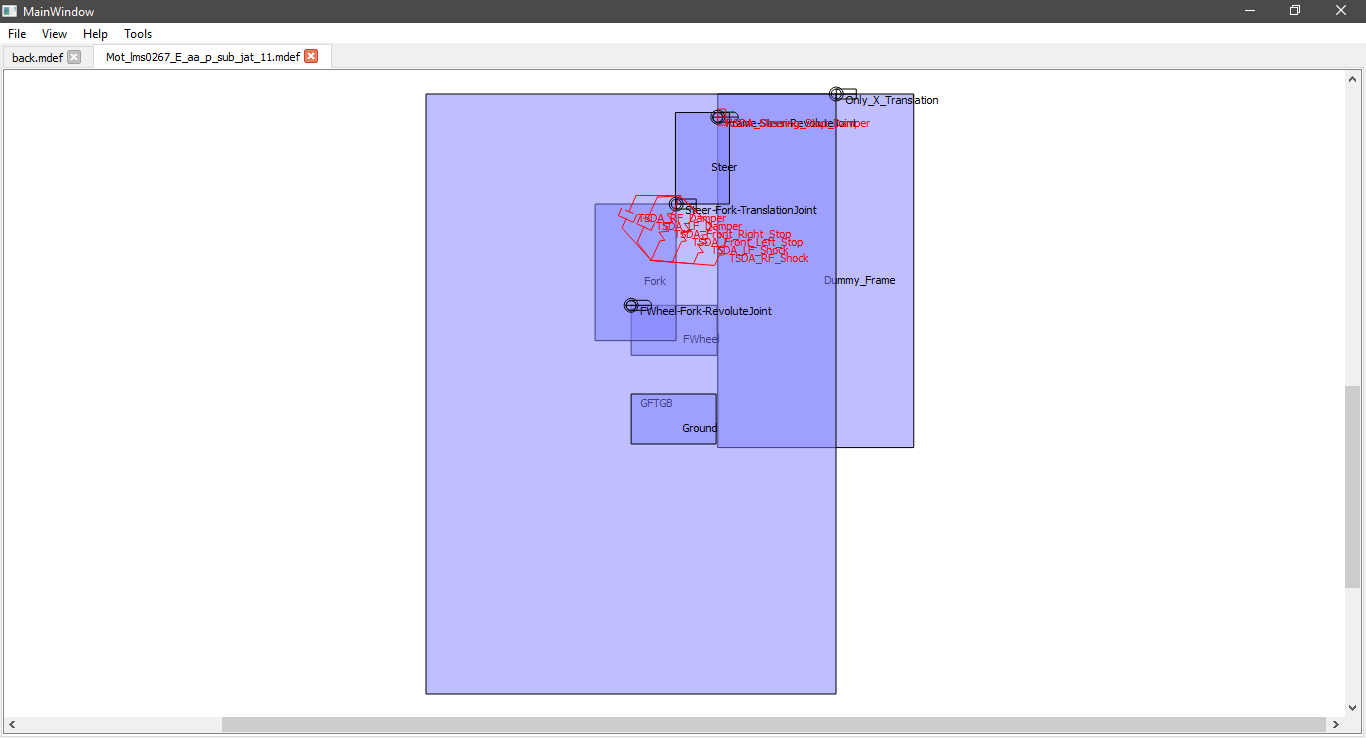
\includegraphics[width=\linewidth]{imagini/implementare/tabs.png}
    \caption{Un model deschis in aplicatie}
    \label{fig:tabs}
\end{figure}

Fișierul reprezentând un model 3D pentru a afișa structura de baza și relațiile dintre elemente 
în sine într-un plan 2D am ales folosirea noțiunii de perspectiva ortografica în care modelul este desenat eliminând 
una dintre cele trei posibile dimensiuni. Astfel se obțin trei perspective individuale pentru afișarea modelului: 
perspectiva laterala eliminând z, perspectiva frontala eliminând x, perspectiva de deasupra eliminând y. Formele 
elementelor din aceasta opțiune au la baza coordonate reale citite din fișier. De exemplu mărimea dreptunghiului 
care reprezinta un Motionbody este calculata în funcție de pozițiile conexiunilor cu alte elemente și centrul de 
greutate. Aceste perspective pot fi alese de utilizator din view->perspectve. Aceasta abordare este folositoare din 
perspectiva utilizatorului doar pentru modele cu un număr mic spre mediu de elemente deoarece pentru modele mai mari 
s-a observat ca datorita structurii lor în multe cazuri existau suprapuneri în oricare dintre cele trei perspective 
făcând înțelegerea modelului din punct de vedere structural mult mai grea.\newline 

\begin{figure}[h]
    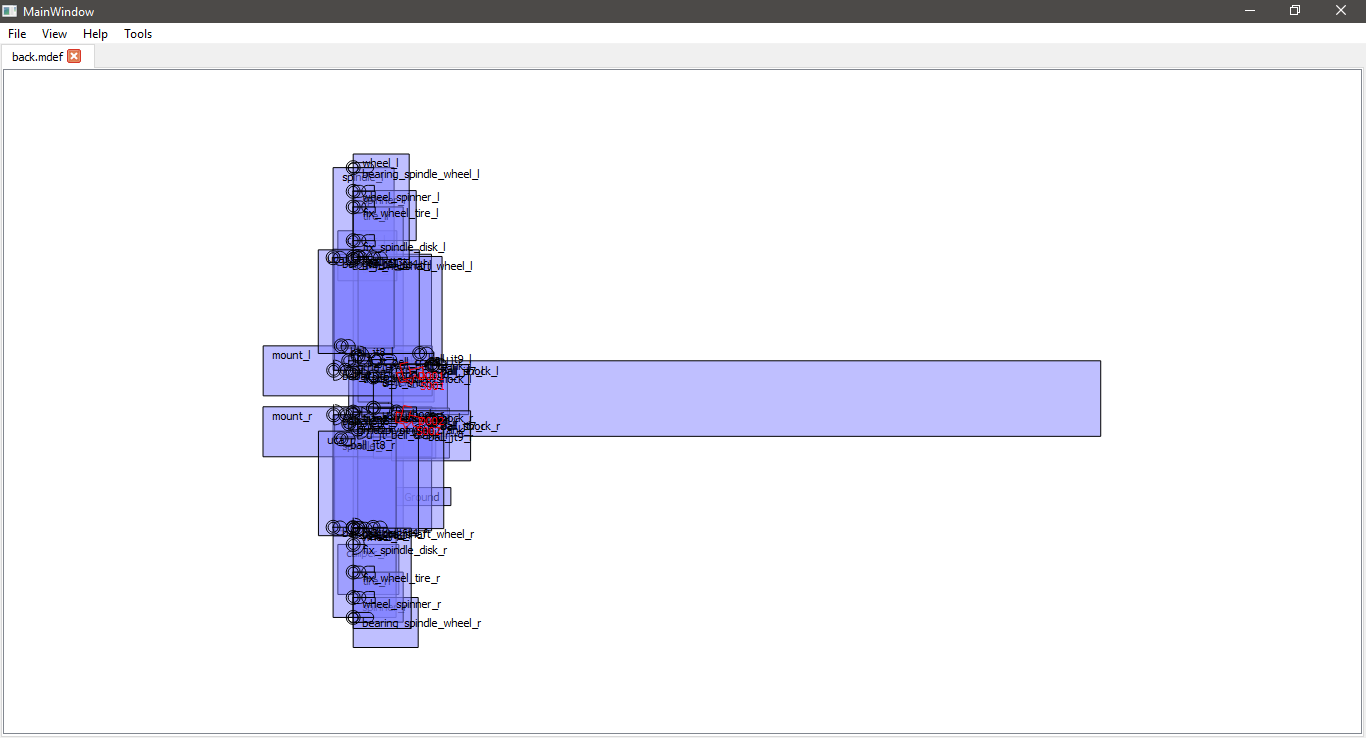
\includegraphics[width=\linewidth]{imagini/implementare/overlapping.png}
    \caption{Un model cu multe suprapuneri intre elemente}
    \label{fig:tabs}
\end{figure}

Pentru cazuri în care apar aceste probleme s-a implementat o structura de graf pentru reprezentarea modelului. 
In comparație cu perspectiva ortografica nu se tine cont de date precum puncte de conexiune sau centru de greutate și se axează strict pe relațiile dintre elemente. 
Folosind un algoritm force-directed de desenare a unui graf obținem o structura mult mai organizata și mai inteligibila, 
însa renunțam la concepte legate silueta modelului. Având în gând un concept prezent în algoritmii force-directed și anume 
cel care garantează ca dacă un graf este planar desenarea lui nu va conține suprapuneri intre muchii și cel mai important 
intre noduri. Totodata si pentru grafuri care nu sunt planare desenarea lui conține un număr minim de suprapuneri intre muchii, 
de multe ori neglijabil, fiind în continuare ușor de înțeles. Opțiunea de graf poate fi aleasa din view->force-directed. 
In aceasta perspectiva se pot evidenția și tipurile de elemente Joint mai bine deoarece nu mai sunt reprezentate ca un punct 
fix dintre doua elemente Motion body ci dintr-o muchie cu un simbol corespondent cu tipul elementului. Totodată din meniul 
de view se poate alege dacă este necesara afișarea fiecărui nume ale elementelor, acest lucru se face din view->show names, 
de unde se poate deselecta cate o căsuță pentru fiecare tip de element.\newline 

\begin{figure}[H]
    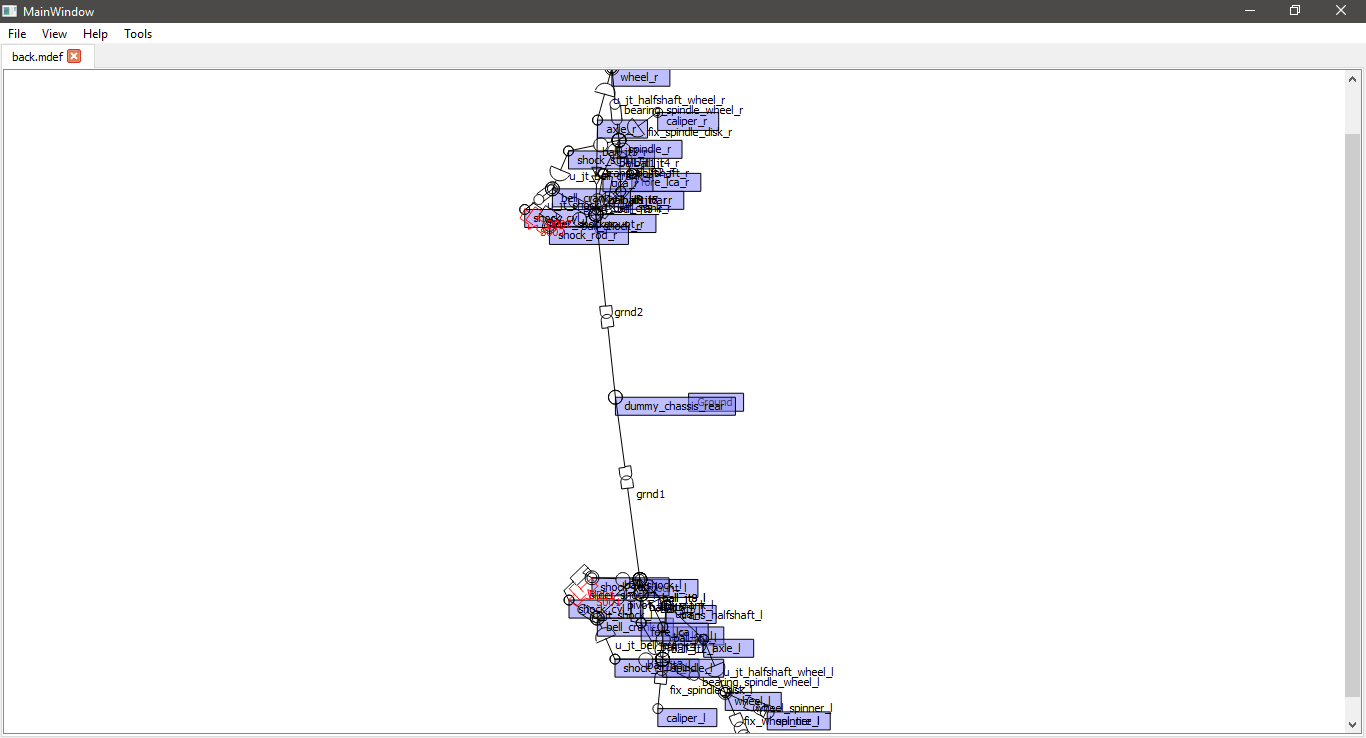
\includegraphics[width=\linewidth]{imagini/implementare/graf.png}
    \caption{Un model deschis in aplicatie sub forma de graf}
    \label{fig:tabs}
\end{figure}

In continuare pentru înțelegerea mai buna a modelului 
au fost implementate niște funcționalități de ajutor. O funcție de căutare pune în evidenta anumite elemente de din model. 
Se poate accesa din help->search de unde este deschisa o noua fereastra cu mai multe opțiuni. Căutarea după un sub srtring 
al cuvântului cheie sau căutarea după întreg cuvântul. Este prezenta și o opțiune de regex prin care utilizatorul poate 
cauta elemente după un anumit șablon. Din aceeași fereastra se poate alege dacă vrem sa cautam doar după anumite tipuri 
de elemente. Dupa ce apăsam search, dacă căutarea a avut succes elementele sunt evidențiate în scena cu o culoare.\newline 

\begin{figure}[H]
    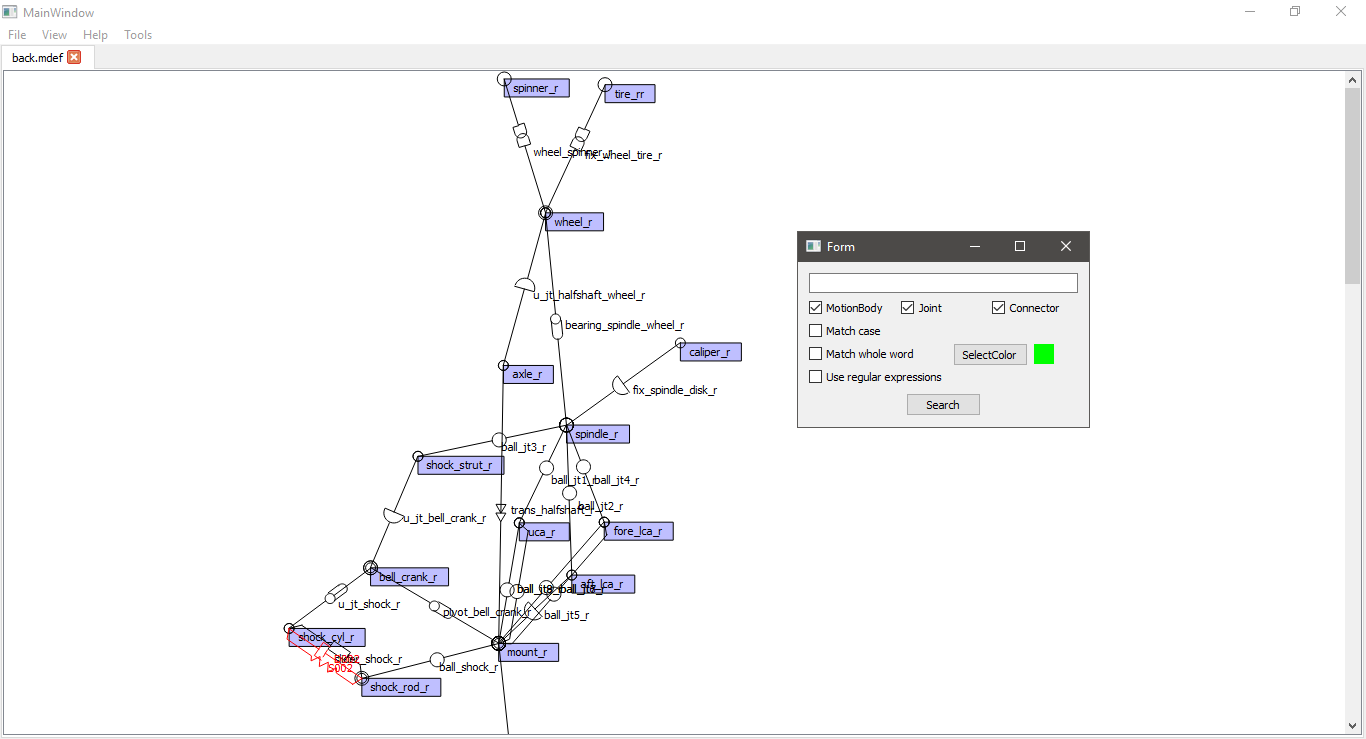
\includegraphics[width=\linewidth]{imagini/implementare/searchwindow.png}
    \caption{Fereastra de cautare}
    \label{fig:tabs}
\end{figure}

O alta funcționalitate este cea a panoului de informații adiționale, acolo sunt afișate date din fișierul .mdef legate de un element 
anume. Aceste informații pot fi accesate prin click dreapta pe un element din scena. Date precum tipul elementului, greutatea, 
dimensiunea și afișarea altor elemente care au legătura cu el.\newline 

\begin{figure}[H]
    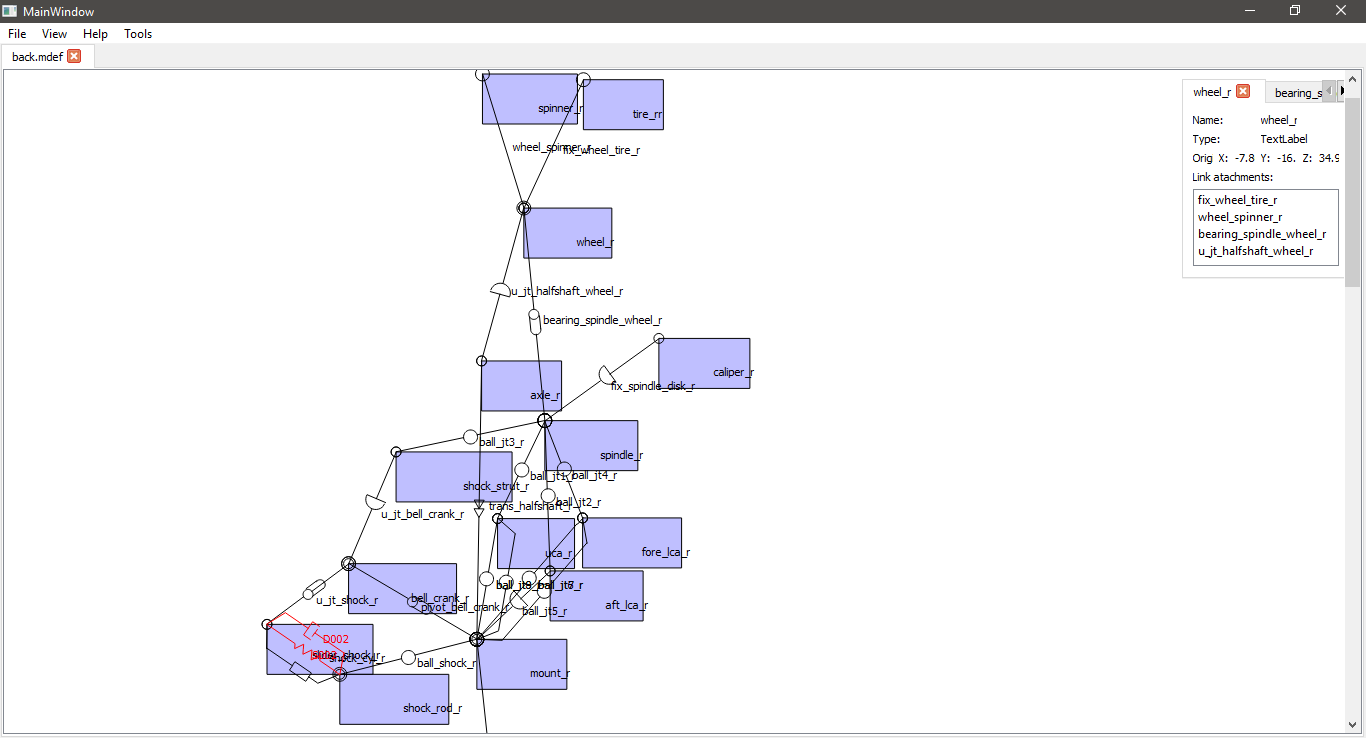
\includegraphics[width=\linewidth]{imagini/implementare/info.png}
    \caption{Panoul cu informatii despre un element Motion body}
    \label{fig:tabs}
\end{figure}

Pentru evidențierea diferențelor dintre versiuni diferite de 
fișiere .mdef a fost implementata funcționalitatea compare models. Se poate accesa din tools->compare models și va deschide 
o noua fereastra de unde utilizatorul poate alege ce modele vrea sa compare dintre cele deschise. Diferențe precum date diferite 
sau chiar lipsa de elemente sunt evidentiate prin colorarea diferita a elementelor.\newline 

\begin{figure}[H]
    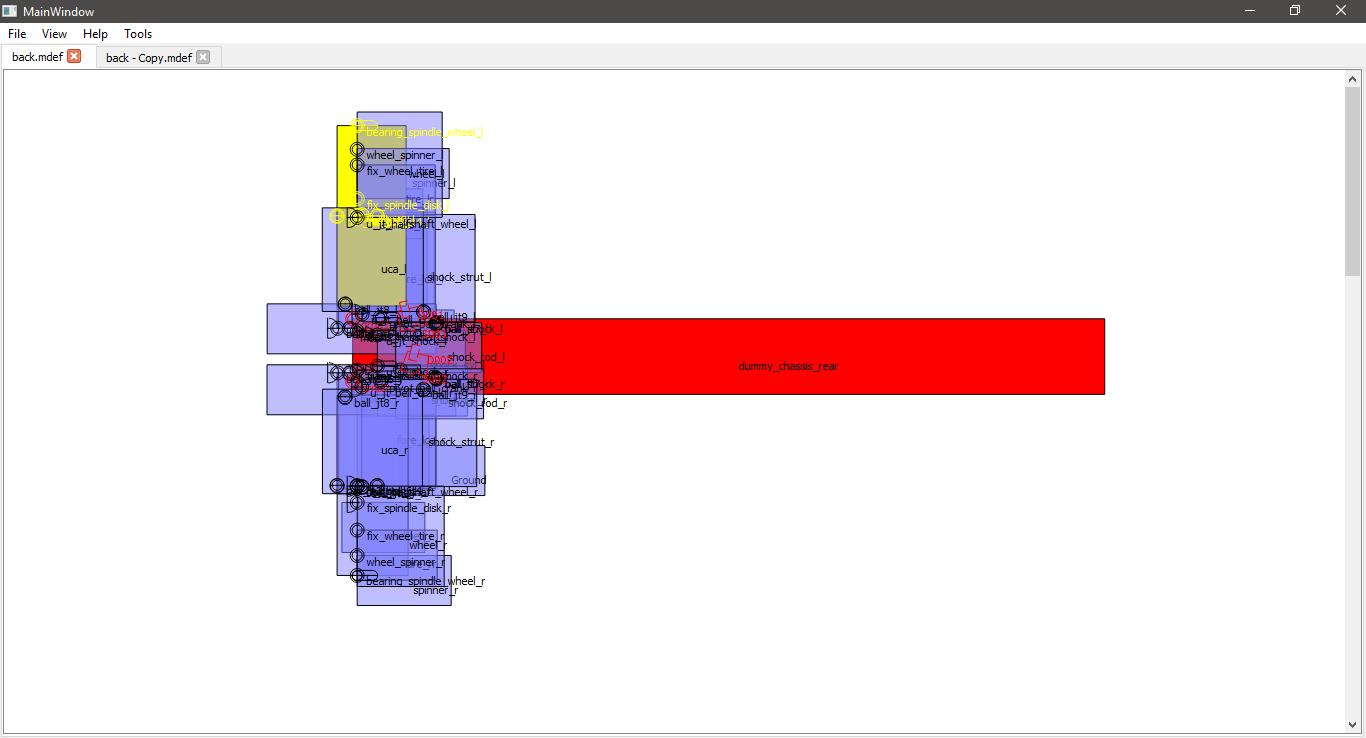
\includegraphics[width=\linewidth]{imagini/implementare/compare.png}
    \caption{Modelul principal comparat cu o alta versiune}
    \label{fig:tabs}
\end{figure}

O alta opțiune de ajutor este cea de legenda. 
Din help->legend se deschide un nou panou care afișează toate simbolurile de elemente Joint și elemente Connectpr pentru ca 
utilizatorul sa înțeleagă mai bine structura modelului.\newline 

\begin{figure}[H]
    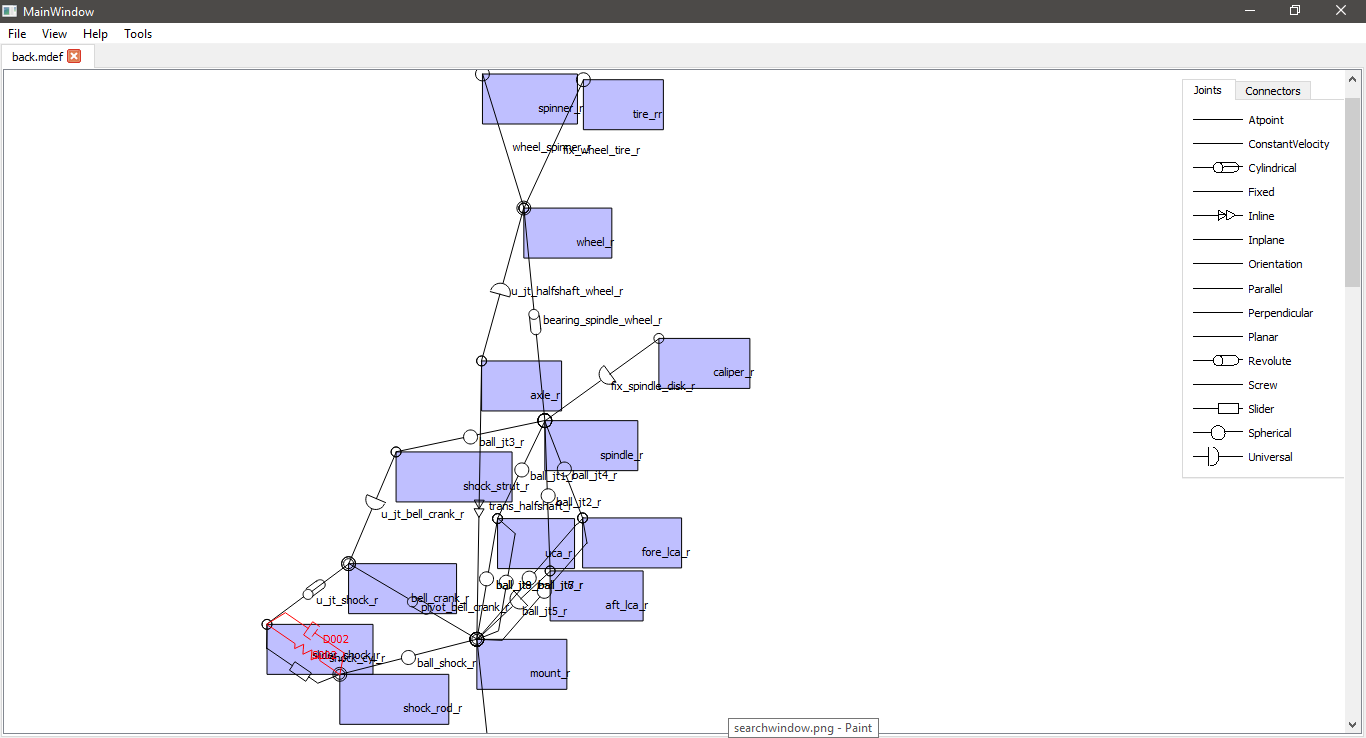
\includegraphics[width=\linewidth]{imagini/implementare/legend.png}
    \caption{Legenda}
    \label{fig:tabs}
\end{figure}

Alte funcționalități minore pentru vizionarea modelului includ funcția 
de zoom și de mutarea elementelor cu mouse-ul. Zoom-ul este necesar pentru modele foarte mari având scopul de a pune în evidenta 
detalii care s-ar observa greu din întregul model. Mutarea elementelor poate fi utila în cazul în care utilizatorul vrea sa 
organizeze în alt fel reprezentarea fișierul.\newline 

\begin{figure}[H]
    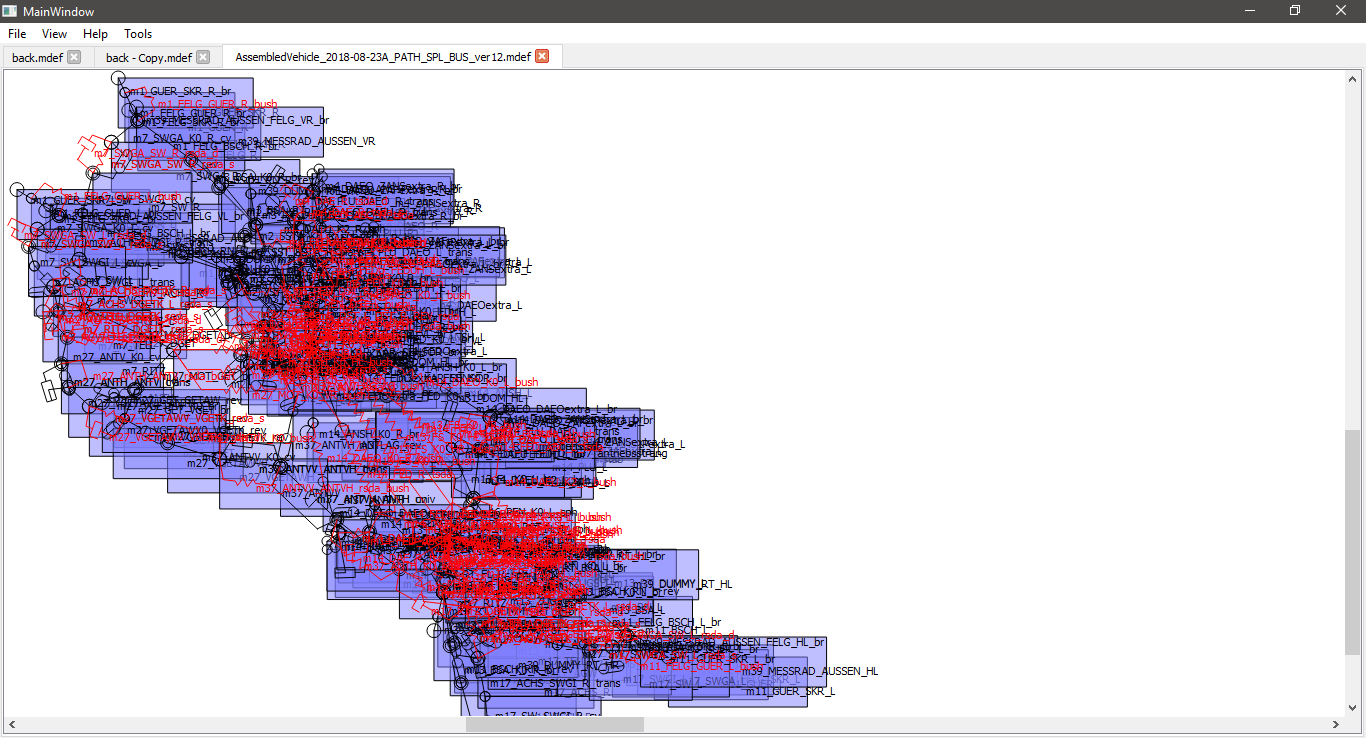
\includegraphics[width=\linewidth]{imagini/implementare/bigmodel.png}
    \caption{Un model cu multe elemente}
    \label{fig:tabs}

    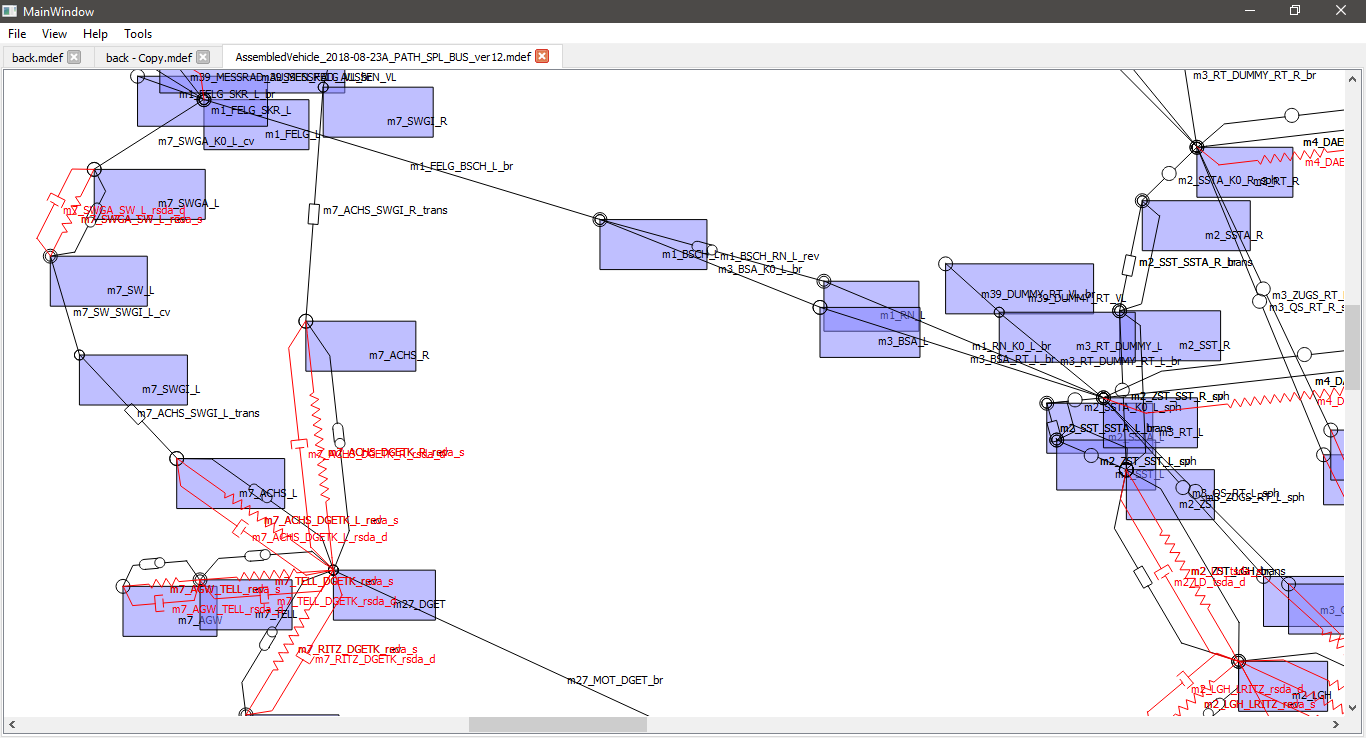
\includegraphics[width=\linewidth]{imagini/implementare/bigmodelzoom.png}
    \caption{Un model cu multe elemente}
    \label{fig:tabs}
\end{figure}

Toate schimbările legate de scena în care se afla toate elementele pot fi salvate 
într-un fișier xml separat. Acest fișier este încărcat automat următoarea data când acel model este încărcat în aplicație. 
Pentru salvare automata file->save sau file->save as pentru salvarea într-un fișier cu nume diferit. Pentru încărcarea explicită 
a salvării file->load. 